% a-project.tex, v-1.0.3 marcoreis baseado no
% abntex2-modelo-trabalho-academico.tex, v-1.9.7 laurocesar
% Copyright 2012-2018 by abnTeX2 group at http://www.abntex.net.br/ 
% 
% This work consists of the files ........
% 
% -----------------------------------------------------------------------------
% Modelo para desenvolvimento de documentação de projetos acadêmicos
% (tese de doutorado, dissertação de mestrado e trabalhos de monografias em geral) 
% em conformidade com ABNT NBR 14724:2011: Informação e documentação. 
% -----------------------------------------------------------------------------
% Opções para a documentação
%
% Fancy page headings 
%\documentclass[fancyheadings, subook]{Classes/a-prj}
%\documentclass[fancyheadings, sureport]{Classes/a-prj}
%
% Fancy chapters and sections headings 
%\documentclass[fancychapter, subook]{Classes/a-prj}
%\documentclass[fancychapter, sureport]{Classes/a-prj}
%
% Fancy page , chapters and sections headings
%\documentclass[fancyheadings, fancychapter, subook]{Classes/a-prj}
\documentclass[fancyheadings, fancychapter, sureport]{Classes/a-prj}
%
% -----------------------------------------------------------------------------
% Alguns comandos para a fancy page headings)
%
% Page header line width
%\footlinewidth{value}
%
% Page footer line width
%\headlinewidth{value}
%
% Page header and footer line width
%\headingslinewidth{value}
%
% Page header and footer lines without text
%\headingslinesonly
%
% The default line width is 0.3pt.
% Set the value to 0pt to remove the page header and/or footer line
%
% -------------------------------------------------------------------------------
% Formato de figuras suportado
% -------------------------------------------------------------------------------
% O formato das figuras depende da forma como o arquivo de saída é gerado.
% As figuras inseridas na pasta Figures serão automaticamente reconhecidas sem
% a necessidade de inserir a extensão do arquivo.
%
% O pdfLaTEX (PDF) suporta figuras com as extensões: pdf, jpg, png e mps.
%
% -------------------------------------------------------------------------------
% Árvore do diretório a-project.tex
%  Diretório
%       \Classes        (requerido)
%       \Figures        (requerido) --------------------------------->
%       \Figures\PDF    (optional)
%       \Figures\JPG    (optional) Figures located within these
%       \Figures\PNG    (optional) folders are searched automatically
%       \Figures\MPS    (optional)  by the a-prj class.
%       \Figures\EPS    (optional)
%       \Figures\PS     (optional) <--------------------------------
%       \Tables         (requerido)
%       \Others         (requerido)
%       \Chapters       (requerido)
%       \Appendices     (optional)
%       \References     (requerido)
%
% -------------------------------------------------------------------------------
% PDF File resumo
\ifpdf
    \hypersetup{
    	backref,
        colorlinks  = true,
        pdftitle    = Modelo de documentação,
        pdfauthor   = {Marco Reis, marco.a.reis@gmail.com},
        pdfsubject  = Mestre em Engenharia,
        pdfcreator  = Subtitulo,
        pdfproducer = PDFLatex,
        pdfkeywords = {documentação, latex, dissertação, tese}}
 \fi
%
% -------------------------------------------------------------------------------
% Relação de pacotes opcionais utilizados
\usepackage[utf8]{inputenc}
\usepackage[brazil]{babel}
\usepackage{longtable}
\usepackage{dcolumn}
\usepackage{multirow}
\usepackage{lscape}
%\usepackage{graphicx}
\usepackage{rotating}
%\usepackage{float,subfigure}
%\usepackage{graphicx, subfigure}
\usepackage{cite}
\usepackage[left=3cm,top=3cm,right=2cm,bottom=2cm]{geometry}
\usepackage[alf]{abntex2cite}
\usepackage{ifpdf}
\usepackage{shadow}
\usepackage{wrapfig}
\usepackage[normalem]{ulem}
\usepackage{makeidx}
\usepackage{yfonts}
\usepackage{algorithm}
\usepackage{algorithmic}
\usepackage{lmodern}
\usepackage[T1]{fontenc}
\usepackage{indentfirst}
\usepackage{color}
\usepackage{microtype}
\usepackage{lipsum}
\usepackage{caption}
\usepackage{subcaption}
%
\makeindex 
\setlength{\LTcapwidth}{\textwidth}
%
\newtheorem{theorem}{Teorema}
\newtheorem{definition}[theorem]{Definição}
%
% -------------------------------------------------------------------------------
% Configurações do pacote backref
\renewcommand{\backrefpagesname}{Citado na(s) página(s):~}
% Texto padrão antes do número das páginas
\renewcommand{\backref}{}
% Define os textos da citação
\renewcommand*{\backrefalt}[4]{
	\ifcase #1 %
		Nenhuma citação no texto.%
	\or
		Citado na página #2.%
	\else
		Citado #1 vezes nas páginas #2.%
	\fi
}
% 
% -------------------------------------------------------------------------------
% Início do documento raiz
\begin{document}
% Definição do título da página
    \university{Centro Universitário SENAI CIMATEC}
	%\faculty{Programa de...}
	%\school{Escola de...}
% 
    %\course{Engenharia Elétrica}
    \typework{Fundamentos de Robótica Móvel}
% 
	%\course{Mestrado em Modelagem Computacional e Tecnologia Industrial}
	%\typework{Disserta\c{c}\~ao de mestrado}
	%\typework{Exame de Qualificação de Mestrado}
% 
	%\course{Engenharia Elétrica}
	%\typework{Tese de doutorado}
	%\typework{Exame de Qualificação de doutorado}
%
% -------------------------------------------------------------------------------
% Informações gerais
    \thesistitle{Desenvolvimento do robô móvel.}
    \hidevolume
    \thesisvolume{Volume 1 of 1}
    \thesisauthor{Michael Faraday}
    \thesisauthorr{John Nash}
    \thesisauthorrr{James Clerk Maxwell}
    \thesisauthorrrr{Nikola Tesla}
    \thesisauthorrrrr{Sir Isaac Newton}
    %\thesisadvisor{Prof. Marco Reis, M.Eng.}
    %\hidecoadvisor
    %\thesiscoadvisor{Marco Reis}
    \thesisdegreetitle{Bacharel em Engenharia}
    \thesismonthyear{Agosto de 2020}
% 
    \maketitlepage
%
% ----------------------------------------------------------------------------
% Inserir Folha de rosto, Nota de estilo, folha de assinaturas, dedicatoria
    \begin{folharosto}

\begin{center}
\theauthor \\
\theauthorr \\
\theauthorrr \\
\theauthorrrr \\
\end{center}
\ \\
\ \\
\ \\
\ \\
\ \\
\begin{spacing}{2}
   \begin{center}
   {\LARGE {\bf \thetitle}}
   \end{center}
\end{spacing}
\ \\
\ \\
\ \\
\vspace*{85mm}
% \begin{flushright}

%    \begin{list}{}{
%       \setlength{\leftmargin}{7.5cm}
%       \setlength{\rightmargin}{0cm}
%       \setlength{\labelwidth}{0pt}
%       \setlength{\labelsep}{\leftmargin}}

%       \item \thetypework apresentada ao \thefaculty, Curso de \thecourse
%       do \theuniversity, como requisito parcial para a obten\c{c}\~ao do
%       t\'itulo de {\bf \thedegreetitle}.

%       \begin{list}{}{
%       \setlength{\leftmargin}{0cm}
%       \setlength{\rightmargin}{0cm}
%       \setlength{\labelwidth}{0pt}
%       \setlength{\labelsep}{\leftmargin}}

%       \item \'Area de conhecimento: Interdisciplinar

%       \item Orientador: \theadvisor
%       \newline \hspace*{2.1cm}  %{\it \theuniversity}

%       \end{list}
%    \end{list}

% \end{flushright}
\ \\
\ \\
\ \\
\ \\
%\begin{spacing}{1.5}
   \begin{center}
   Salvador \par
   \theuniversity \par
   2020
   \end{center}
%\end{spacing}

\end{folharosto}

    %\begin{notaestilo}
Esta \thetypeworkthree foi elaborada considerando as normas de
estilo (i.e. est\'eticas e estruturais) propostas aprovadas pelo
colegiado do \thefacultytwo e est\~ao dispon\'iveis em formato
eletr\^onico ({\it download} na P\'agina Web
http:$//$ead.fieb.org.br$/$portal\_faculdades$/$dissertacoes-e-teses-mcti.html
ou solicita\c{c}\~ao via e-mail \`a secretaria do
programa) e em formato impresso somente para consulta. \\

Ressalta-se que o formato proposto considera diversos itens das
normas da Associa\c{c}\~ao Brasileira de Normas T\'ecnicas (ABNT),
entretanto opta-se, em alguns aspectos, seguir um estilo pr\'oprio
elaborado e amadurecido pelos professores do programa de
p\'os-gradua\c{c}\~ao supracitado.

\end{notaestilo}

    %\begin{folhaassinaturas}

%\thispagestyle{empty}

\def\signature#1#2{\parbox[b]{1in}{\smash{#1}\vskip12pt}
\hfill \parbox[t]{3in}{\shortstack{\vrule width 3in height
0.4pt\\\small#2}}}

\def\InstituicaoMembro#1#2{\parbox[b]{1in}{\smash{#1}\vskip12pt}
\hfill \parbox[t]{3in}{\shortstack{\vrule width 3in \\\small#2}}}

\def\signaturepage{%

    \begin{spacing}{1.5}
        \begin{center}
        {\LARGE \theuniversity} \\
        {\large \thefaculty} \\
        {\large \thecourse} \\
        \end{center}
    \end{spacing}

   \vskip 0.25in plus 0.4in minus 0.1in

    \begin{spacing}{1.5}
        \begin{sloppypar}
        A Banca Examinadora, constitu\'ida pelos professores abaixo
        listados, leram e recomendam a aprova\c{c}\~ao [com distin\c{c}\~ao] da
        \thetypeworktwo, intitulada ``\thetitle",
        apresentada no dia (dia) de (m\^es) de (ano), como requisito
        parcial para a obten\c{c}\~ao do t\'itulo de {\bf \thedegreetitle}.\\
        \end{sloppypar}
    \end{spacing}

    \def\sigskip{\vskip0.15in plus 0.2in minus 0.1in}
    \def\beginskip{\vskip0.3875in plus 0.2in minus 0.1in}

    \beginskip
    \signature{Orientador:}{Prof. Dr. \theadvisor} \\
    \InstituicaoMembro{}{\theuniversity} \\

    \sigskip
    \beginskip
    \signature{Membro externo da Banca:}{Prof. Dr. Nome completo} \\
    \InstituicaoMembro{}{Institui\c{c}\~ao do membro da banca} \\

    \sigskip
    \beginskip
    \signature{Membro externo da Banca:}{Prof. Dr. Nome completo} \\
    \InstituicaoMembro{}{Institui\c{c}\~ao do membro da banca} \\

    %\sigskip
    %\beginskip
   % \signature{Membro interno da Banca:}{Prof. Dr. Nome completo} \\
   % \InstituicaoMembro{}{Institui��o do membro da banca} \\

    \vfill
    \newpage
    \setcounter{page}{3}
}
%*********************************************************************


\signaturepage


\end{folhaassinaturas}

    %\include{Others/dedicatoria}
    %\include{Others/agradecimentos}
%
% ----------------------------------------------------------------------------
% Resumo/abstract, sumário e siglas
    \begin{romanpagenumbers}
        \begin{thesisresumo}
Escreva aqui o resumo da disserta\c{c}\~ao, incluindo os contextos geral e espec\'ifico, dentro dos quais a pesquisa foi realizada, o objetivo da pesquisa, assun\c{c}\~ao filos\'ofica, os m\'etodos de pesquisa usados e as poss\'iveis contribui\c{c}\~oes que o que \'e proposto pode trazer \`a sociedade.

\ \\

% use de três a cinco palavras-chave

\textbf{Palavras-chave}: Palavra-chave 1, Palavra-chave 2, Palavra-chave 3, Palavra-chave 4, Palavra-chave 5

\end{thesisresumo}

        \begin{thesisabastract}
Escreva aqui, em ingl\^es, o resumo da disserta\c{c}\~ao, incluindo os contextos geral e espec\'ifico, dentro dos quais a pesquisa foi realizada, o objetivo da pesquisa, assun\c{c}\~ao filos\'ofica, os m\'etodos de pesquisa usados e as poss\'iveis contribui\c{c}\~oes que o que \'e proposto pode trazer \`a sociedade. 

\ \\

% use de tr�s a cinco palavras-chave

\textbf{Keywords}: Keyword 1, Keyword 2, Keyword 3, Keyword 4, Keyword 5

\end{thesisabastract}

        % Make list of contents, tables and figures
        \thesiscontents
        %Include other required section
        %\begin{thesisabbreviations}
\begin{footnotesize}
\begin{longtable}[l]{p{2cm}l}
  tprax   \dotfill & \thefaculty \\
  WWW       \dotfill &  World Wide Web \\
\end{longtable}
\end{footnotesize}
\end{thesisabbreviations}

        %\begin{thesissymbols}
\begin{footnotesize}
\begin{longtable}[l]{p{2cm}l}
  $\partial$   \dotfill  & Bla bla bla \\
  $\prod$       \dotfill & ble ble ble \\
  $\partial$   \dotfill  & Bla bla bla \\
  $\prod$       \dotfill & ble ble ble \\
  $\partial$   \dotfill  & Bla bla bla \\
  $\prod$       \dotfill & ble ble ble \\
  $\partial$   \dotfill  & Bla bla bla \\
  $\prod$       \dotfill & ble ble ble \\
  $\partial$   \dotfill  & Bla bla bla \\
  $\prod$       \dotfill & ble ble ble \\
  $\partial$   \dotfill  & Bla bla bla \\
  $\prod$       \dotfill & ble ble ble \\
  $\partial$   \dotfill  & Bla bla bla \\
  $\prod$       \dotfill & ble ble ble \\
  $\partial$   \dotfill  & Bla bla bla \\
  $\prod$       \dotfill & ble ble ble \\
  $\partial$   \dotfill  & Bla bla bla \\
  $\prod$       \dotfill & ble ble ble \\
  $\partial$   \dotfill  & Bla bla bla \\
  $\prod$       \dotfill & ble ble ble \\
  $\partial$   \dotfill  & Bla bla bla \\
  $\prod$       \dotfill & ble ble ble \\
  $\partial$   \dotfill  & Bla bla bla \\
  $\prod$       \dotfill & ble ble ble \\
  $\partial$   \dotfill  & Bla bla bla \\
  $\prod$       \dotfill & ble ble ble \\
  $\partial$   \dotfill  & Bla bla bla \\
  $\prod$       \dotfill & ble ble ble \\
  $\partial$   \dotfill  & Bla bla bla \\
  $\prod$       \dotfill & ble ble ble \\
  $\partial$   \dotfill  & Bla bla bla \\
  $\prod$       \dotfill & ble ble ble \\
  $\partial$   \dotfill  & Bla bla bla \\
  $\prod$       \dotfill & ble ble ble \\
  $\partial$   \dotfill  & Bla bla bla \\
  $\prod$       \dotfill & ble ble ble \\
  $\partial$   \dotfill  & Bla bla bla \\
  $\prod$       \dotfill & ble ble ble \\          
\end{longtable}
\end{footnotesize}
\end{thesissymbols}

        %Switch the page numbering back to the default format
    \end{romanpagenumbers}
%
% ---------------------------------------------------------------------------
% Include thesis chapters
    \parskip=\baselineskip
    \chapter{Introdução}
\label{chap:intro}

Este pode ser um parágrafo citado por alguém \cite{Barabasi2003-1}.

%--------- NEW SECTION ----------------------
\section{Objetivos}
\label{sec:obj}

Nesta se\c{c}\~ao os objetivos principal (tamb\'em
pode-se se utilizar a palavra meta) da monografia de
gradua\c{c}\~ao ou especializa\c{c}\~ao, disserta\c{c}\~ao de
mestrado ou tese de doutorado s\~ao apresentados.


\subsection{Objetivos Específicos}
\label{ssec:objesp}

Nesta se\c{c}\~ao os objetivos espec\'ificos (tamb\'em
pode-se se utilizar a palavra meta) da monografia de
gradua\c{c}\~ao ou especializa\c{c}\~ao, disserta\c{c}\~ao de
mestrado ou tese de doutorado s\~ao apresentados.


%--------- NEW SECTION ----------------------
\section{Justificativa}
\label{sec:justi}

O pesquisador/estudante deve apresentar os aspectos mais
relevantes da pesquisa ressaltando os impactos (e.g. cient\'ifico,
tecnol\'ogico, econ\^omico, social e ambiental) que a pesquisa
causar\'a. Deve-se ter cuidado com a ingenuidade no momento em que
os argumentos forem apresentados.




%--------- NEW SECTION ----------------------
\section{Organização do documento}
\label{section:organizacao}

Este documento apresenta $5$ capítulos e está estruturado da seguinte forma:

\begin{itemize}

  \item \textbf{Capítulo \ref{chap:intro} - Introdução}: Contextualiza o âmbito, no qual a pesquisa proposta está inserida. Apresenta, portanto, a definição do problema, objetivos e justificativas da pesquisa e como este \thetypeworkthree está estruturado;
  \item \textbf{Capítulo \ref{chap:fundteor} - Fundamentação Teórica}: XXX;
  \item \textbf{Capítulo \ref{chap:mat} - Materiais e Métodos}: XXX;
  \item \textbf{Capítulo \ref{chap:result} - Resultados}: XXX;
  \item \textbf{Capítulo \ref{chap:conc} - Conclusão}: Apresenta as conclusóes, contribuições e algumas sugestões de atividades de pesquisa a serem desenvolvidas no futuro.

\end{itemize}

    \chapter{Fundamentação Teórica}
\label{chap:fundteor}

% \begin{flushright}

%    \begin{list}{}{
%       \setlength{\leftmargin}{4.5cm}
%       \setlength{\rightmargin}{0cm}
%       \setlength{\labelwidth}{0pt}
%       \setlength{\labelsep}{\leftmargin}}
%       \item Quanto maior for a rapidez de transformação de uma
%       sociedade, mais temporárias são as necessidades
%       individuais. Essas flutuaçõess tornam ainda mais acelerado
%       o senso de turbilh da sociedade.

%       \begin{list}{}{
%       \setlength{\leftmargin}{0cm}
%       \setlength{\rightmargin}{0cm}
%       \setlength{\labelwidth}{0pt}
%       \setlength{\labelsep}{\leftmargin}}
%       \item (Alvin Toffler)
%       \end{list}
%    \end{list}
% \end{flushright}

% \begin{flushright}
%   Quanto maior for a rapidez de transformação de uma \\
%   sociedade, mais temporárias são as necessidades \\
%   individuais. Essas flutuações tornam ainda mais \\
%   acelerado o senso de turbilhão da sociedade. \\
%   \ \\
%   (Alvin Toffler)
% \end{flushright}

%--------- NEW SECTION ----------------------
\section{Estudo da Odometria}
Informações relacionadas a localização são essenciais em diversas aplicações relacionadas à robótica móvel nos dias atuais. Determinar a posição em um ambiente, dado um mapa daquele ambiente e dados sensoriais locais, pode ser a definição de localização para um robô móvel. Isto foi um dos grandes problemas passados na área de robótica e ainda nos tempos atuais é um campo de bastante estudo.
Como uma das possíveis soluções para este problema, foi apresentado o cálculo baseado em medidas odométricas. Odometria nada mais é que o uso de dados capturados por sensores de movimento e assim então estimar mudança de posição com o tempo. É altamente usada na robótica por alguns robôs com rodas ou legados para estimar sua posição relativa de um ponto de partida. Entretanto, para um uso efetivo desta tecnologia é necessário uma captura rápida e precisa de dados, calibração de instrumentos e processamento.

Um sensor interessante para captura de dados como velocidade e posição é o sensor de WiFi. Um exemplo prático foram pesquisadores da Universidade da Carolina do Norte desenvolveram um meio para capturar a velocidade e distância em ambientes indoor através de um sensor WiFi. Este sensor funciona como um sensor de velocidade para assim rastrear com precisão o quão longe algo se moveu; exatamente como um sonar mas usando ondas de rádio ao invés de ondas de som.
\cite{Diego2016}

\begin{itemize}

    \item \textbf{Trilateração}: métodos que utilizam as propriedades geométricas do triângulo para encontrar a posição do alvo. Diferente da triangulação, este processo determina o posicionamento a partir de 3 pontos de referência diferentes, assim como acontece em sistemas de GPS(Global Positioning System). Podem ser divididos em métodos por lateração e angulação.;
    
    \begin{itemize}
        \item \textbf{Lateração} estima a posição do objeto através da leitura de distâncias a partir de múltiplos pontos de referência.
        
        \begin{itemize}
            \item \textbf{TOA (Time Of Arrival)}: a distância do alvo móvel até a unidade medidora
            é diretamente proporcional ao tempo de propagação; 
            \item \textbf{TDOA (Time Difference Of Arrival)}: este método busca determinar a posição relativa do transmissor através da diferença de tempo entre o envio até as unidades recptoras.
            \item \textbf{Baseadas em RSS (Received Signal Strength)}: método que calcula a distância baseada na atenuação da força do sinal entre o emissor e o receptor. Os métodos baseados em RSS, assim como os dois anteriores necessitam da inexistência de obstáculos físicos entre os participantes da conversa.
            \item \textbf{RTOF (Reflection Time Of Flight)}: este método utiliza do valor de Time of Flight, ou tempo de voo do sinal, para estimar a posição. O tempo de voo do sinal 
            \item \textbf{RSP (Received Signal Phase)}: utiliza a diferença de fase no sinal das portadoras (de telefonia, por exemplo) para estimar a posição.
        \end{itemize}

        \item \textbf{Angulação}: estima a posição do alvo através da interseção de vários pares de
        ângulos das linhas de direção. Cada linha é formada pelo raio do círculo de alcance
        do sinal partindo da estação base ao receptor móvel.

    \end{itemize}

    \item \textbf{Análise de Cenário}: refere-se aos métodos que primeiro recuperam características do sinal de Wi-Fi no ambiente e depois estimam a localização de um objeto através da relação da informação do sinal atual junto ao sinal adquirido anteriormente. 

\end{itemize}

A complexidade das iterações do sinal de Wi-Fi em ambientes fechados favorece a utilização dos métodos baseados em mapas, orientados por dados de intensidade do sinal.
Deixando a utilização da odometria por Wi-Fi menos optável. Biswas e Veloso propôem um método onde a posição é estimada em um processo de duas etapas. Chamados de fase de aprendizado e fase de localização.
A primeira define-se como a construção de um mapa na forma de um grafo, onde cada vértice armazena um conjunto de médias e desvios padão das forças do sinal de cada ponto de acesso Wi-Fi mensurada naquela posição e cada aresta do mapa representa um caminho possível para movimentação do robô.
E a segunda, utiliza um algoritmo que se baseia em filtro de partículas para a obtenção da posição do robô, relacionando as medições do sinal Wi-Fi recebido durante a movimentação com os valores previamente populados no mapa.\cite{Biswas2010}

%--------- NEW SECTION ----------------------
\section{Aplicação na Robótica}
\label{sec:ass1}
\lipsum[1]

%---------------picture------------------------------------
% \begin{figure}
%     \centering
%     \subfigure[Figure A]{\label{fig:a}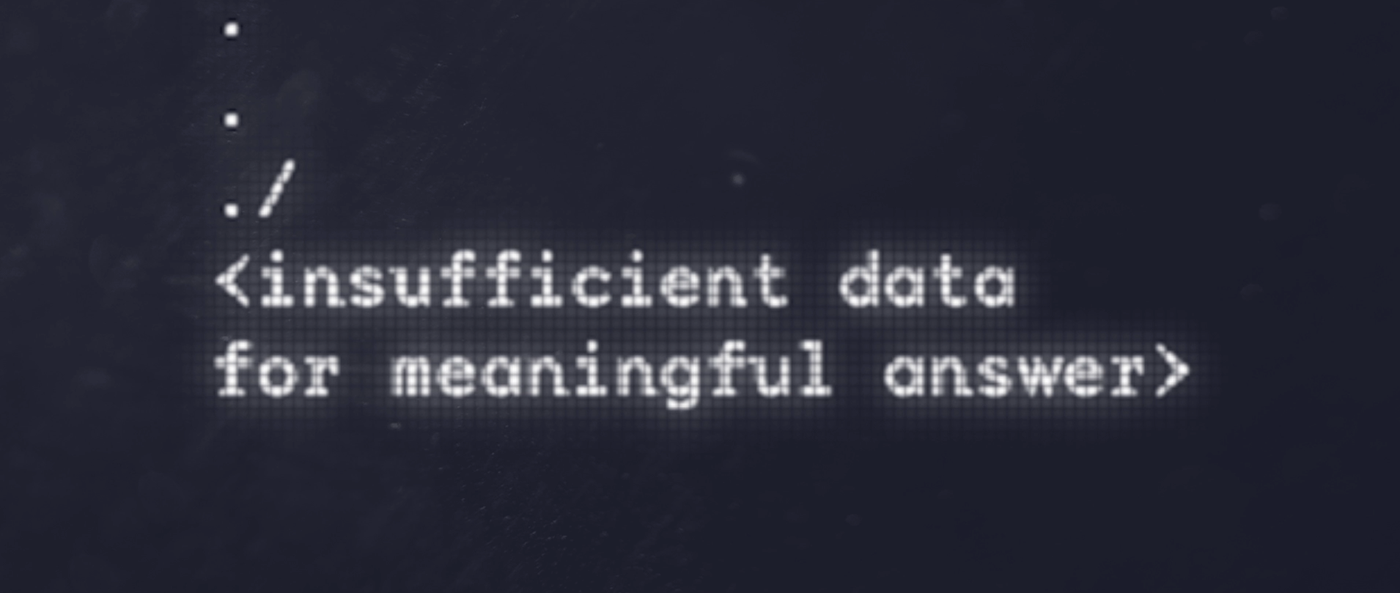
\includegraphics[width=60mm]{./lq}}
%     \subfigure[Figure B]{\label{fig:b}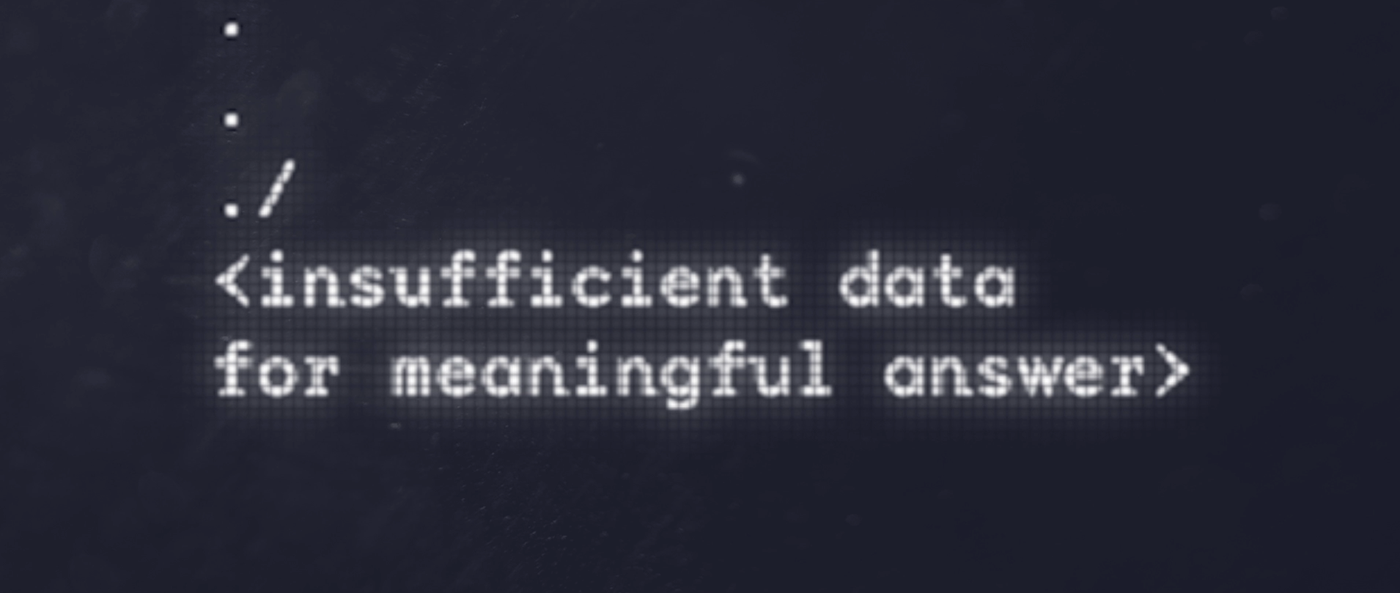
\includegraphics[width=60mm]{./lq}}
%     \subfigure[Figure C]{\label{fig:c}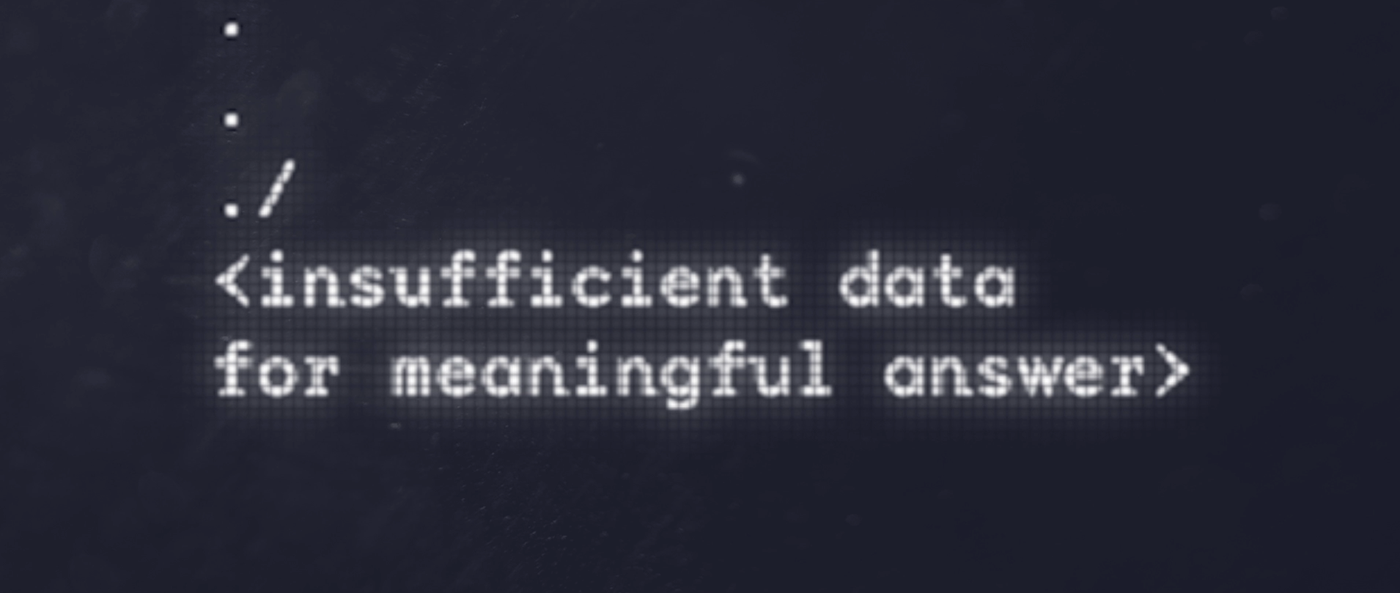
\includegraphics[width=\textwidth]{./lq}}
%     \caption{Three simple graphs}
%     \label{fig:three graphs}
% \end{figure}
%----------------------------------------------------------


    \chapter{Materiais e Métodos}
\label{chap:mat}
\lipsum[1]

\section{Metodologia}
\label{sec:met}
\lipsum[1]

%--------- NEW SECTION ----------------------
\section{Interface do Usuário}
\label{sec:ui}
\lipsum[1]

%--------- NEW SECTION ----------------------
\section{Simulação do sistema}
\label{sec:sim}
\lipsum[2-4]


    \chapter{Resultados}
\label{chap:result}
Importante sempre ter um parágrafo introdutório para explicar os resultados encontrados.

%--------- NEW SECTION ----------------------
\section{Testes unitários}
\label{sec:testu}
\lipsum[1]

\section{Integração do sistema}
\label{sec:intsis}
\lipsum[1]

%--------- NEW SECTION ----------------------
\section{Testes integrados}
\label{sec:testi}
\lipsum[1]








    \chapter{Conclusão}
\label{chap:conc}


Com essa pesquisa conclui-se que a aplicação de sensor Wi-Fi para odometria indoor na robotica movel é viavel quando unido com outros sensores, como é mostrado por \cite{Diego2016} que 
utiliza 2 sensores al\'em do sensor Wi-Fi, a camera e o compasso digital. Na pesquisa de \cite{Diego2016} foram realizadas análises com dados reais e dados simulados com relação a precisão de trajetória dos algoritmos envolvidos na odometria visual. As análises da precisão entre trajetória real executada pelo robô e a obtida
pelo robô mostraram uma margem de erro próximo a 2,0 metros que pode ser considerada
aceitável dependendo do tamanho do robô utilizado.

% \textbf{Conclus\~oes}.


% Chegou a hora de apresentar o apanhado geral sobre o trabalho de
% pesquisa feito, no qual s\~ao sintetizadas uma s\'erie de
% reflex\~oes sobre a metodologia usada, sobre os achados e
% resultados obtidos, sobre a confirma\c{c}\~ao ou recha\c{c}o da
% hip\'otese estabelecida e sobre outros aspectos da pesquisa que
% s\~ao importantes para validar o trabalho. Recomenda-se n\~ao
% citar outros autores, pois a conclus\~ao \'e do pesquisador.
% Por\'em, caso necess\'ario, conv\'em cit\'a-lo(s) nesta parte e
% n\~ao na se\c{c}\~ao seguinte chamada \textbf{Conclus\~oes}.


% \section{Considerações finais}
% \label{sec:consid}

% Brevemente comentada no texto acima, nesta se\c{c}\~ao o
% pesquisador (i.e. autor principal do trabalho cient\'ifico) deve
% apresentar sua opini\~ao com respeito \`a pesquisa e suas
% implica\c{c}\~oes. Descrever os impactos (i.e.
% tecnol\'ogicos,sociais, econ\^omicos, culturais, ambientais,
% políticos, etc.) que a pesquisa causa. N\~ao se recomenda citar
% outros autores.


    % include more chapters ...
%
% ----------------------------------------------------------------------------
% Include thesis appendices
    \begin{thesisappendices}
        % Thesis Appendix -------------------------------------------------------

\chapter{Diagramas mecânicos}
\label{Append:diagmec}



        % Thesis Appendix -------------------------------------------------------

\chapter{Diagramas eletro-eletrônicos}
\label{Append:diagele}



        % Thesis Appendix -------------------------------------------------------

\chapter{Logbook}
\label{Append:log}



    \end{thesisappendices}
%
% ----------------------------------------------------------------------------
% Configurar as referencias bibliograficas
	\renewcommand\bibname{Referências}
    \addcontentsline{toc}{chapter}{Referências}
    \bibliography{References/referencias}
%
% ----------------------------------------------------------------------------
% Finishing him
    \include{Others/ultimafolha}
\end{document}
%
% -------------------------------------------------------------------------------
% Aqui termina a formatação para o documento.
% In God We Trust. All Other Bring Data. 
%
% -------------------------------------------------------------------------------